\section{Results - Titan \label{sec:results}}

The following results are split into three main sections. We firstly present solutions to the LTEs using Rayleigh friction and compare dissipation between the analytical and numerical solutions in section \ref{subsec:result_rayleigh}. Section \ref{subsec:result_bottom} then presents purely numerical results for dissipation using only bottom friction. Finally, dissipation in the bottom friction case is compared to analytical scaling laws derived by \citet{chen2013tidal} in section \ref{subsec:scaling}.

\subsection{Rayleigh Friction \label{subsec:result_rayleigh}}

The primary task of ODIS is to solve the LTE on a sphere, and it is from these solutions that dissipation is derived. Thus, a useful starting point are the velocity and displacement solutions to the LTEs rather than purely concerning the reader with the average tidal dissipation over an orbital period. 

Figure \ref{fig:LTE_solns} illustrates numerical solutions to the LTE, at periapse, for different components of the tidal potential on Titan. Surface displacement, $\eta$, is illustrated on the left, whereas velocity, $\bm{u}$, is on the right. The colour scale in the velocity figures represents the velocity's magnitude, $\left| \bm{u} \right|$, Arrows indicate the direction of flow. The tidal forcing applied is, from a) to c), the eccentricity tide, obliquity tide, and both tides combined together, respectively. All plots are for the ``canonical'' $400 \, \si{\metre}$ ocean outlined by \citet{sagan1982tide} for best comparison with \citet{sears1994tidal,sears1995tidal,sohl1995tidal}.

Surface displacement in Figure \ref{fig:LTE_a} shows a classic tidal bulge, centered on the Saturnian ($\phi = 0^{\circ}$) and sub-Saturian ($\phi = 180^{\circ}$) points. Maximum displacement is over $8$ metres. Away from the tidal bulge, displacement drops below the equilibrium level to less than $4$ metres. The corresponding flow shows convergence and divergence at the longitudinal positions of steepest gradient in the displacement field. Fastest flow occurs at the maxima and minima of the displacement.

The obliquity tide shows markedly different displacement and flow patterns than the eccentricity tide (Figure \ref{fig:LTE_b}). Displacement is now anti-symmetric about the equator. Notably, the longitudinal positions of maxima and minima are offset from the Saturnian and sub-Saturnian points. The tide raised by the obliquity tidal potential is also an order of magnitude less than the eccentricity tide. Flow is mainly poleward, converging south of the equator on the Saturn-facing hemisphere, and north of the equator on the opposite hemisphere.

The final plot in figure \ref{fig:LTE_solns} is the solution under the full tidal potential. In many ways, it is similar to the eccentricity tide. Yet, the addition of the obliquity tide adds significant equatorial asymmetry to the solutions. This asymmetry is particularly noticeable in the velocity plot on the right hand side of Figure \ref{fig:LTE_c}, where the areas of fastest flow are skewed north and south of the equator, unlike in Figure \ref{fig:LTE_a}. This is also evident in the displacement field, where the tidal bulge maximum does not lie directly on the equator.

Comparisons made between the results in Figure \ref{fig:LTE_solns} and the analytical solutions show excellent agreement for this test case.

The simulations used in Figure \ref{fig:LTE_solns} were run from undisturbed initial conditions: \hbox{$\eta = 0 \, \si{\metre}$} and \hbox{$\bm{u} = (0,0) \, \si{\metre\per\second}$}. Consequently, there is some start-up time required for the model to converge into its periodic equilibrium, as noted by \citet{sears1995tidal}. Figure \ref{fig:diss} illustrates this issue. From top to bottom, the figure shows orbitally averaged dissipation against time for the eccentricity-libration, eccentricity-radial, and obliquity tides.  The solid lines represent the average dissipation over each orbit in the numerical model, while the dashed lines indicate the analytical time-averaged dissipation value. 

Initially, the time-averaged dissipation for each model differs from the analytical value. The obliquity tide starts with lower dissipation (fig. \ref{fig:diss_c}), whereas the two components of the eccentricity tide begin with higher dissipation (fig. \ref{fig:diss_a} and \ref{fig:diss_b}). With progressing simulation time, the numerical model then converges onto the analytical value. After 100 Titan orbits, all model values are within $1 \si{\percent}$ of the analytical solution. 

\begin{figure}[!t]
\centering
\begin{subfigure}{\linewidth}
\centering
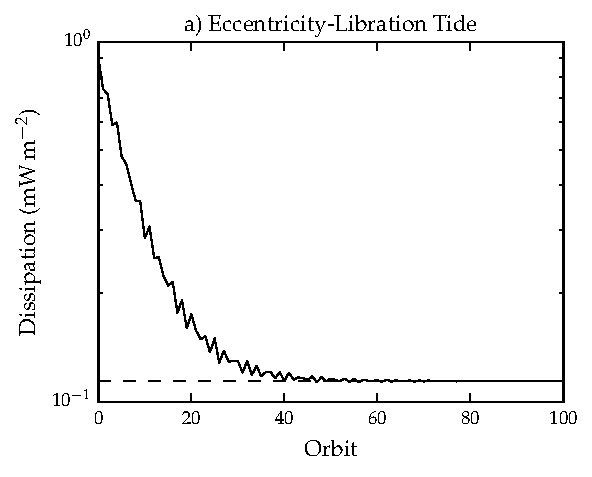
\includegraphics[width=0.8\linewidth]{Figures/ecc_lib_diss}
\subcaption{\label{fig:diss_a}}
\end{subfigure}\vspace*{-0.7cm}
\begin{subfigure}{\linewidth}
\centering
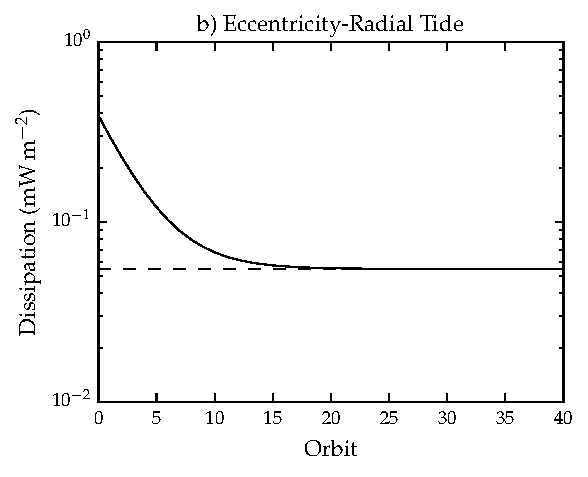
\includegraphics[width=0.8\linewidth]{Figures/ecc_rad_diss}
\subcaption{\label{fig:diss_b}}
\end{subfigure}\vspace*{-0.7cm}
\begin{subfigure}{\linewidth}
\centering
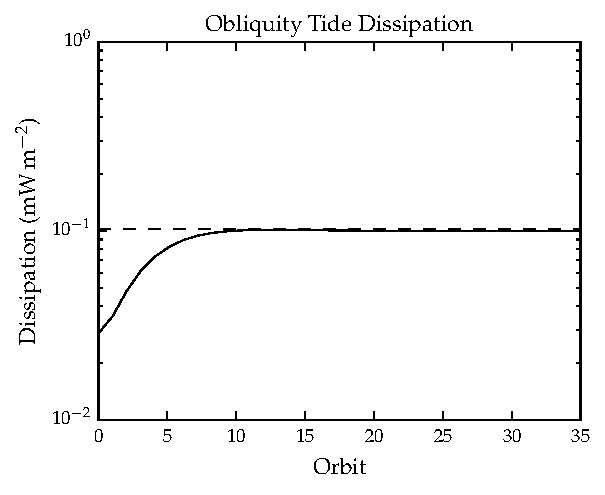
\includegraphics[width=0.8\linewidth]{Figures/obliq_diss}
\subcaption{\label{fig:diss_c}}
\end{subfigure}
\vspace*{-0.8cm}
\caption{Average dissipation over each orbit under the eccentricity-libration, eccentricity-radial, obliquity tides for $h = 400 \, \si{\metre}$ and $\alpha = 1 \times 10^{-7} \, \si{\per\second}$ from undisturbed inital conditions on Titan. The dashed lines represent analytical solutions for the time-averaged dissipation. Solid lines are the numerical solution. \label{fig:diss}}
\end{figure}

%\begin{table}[!b]
\footnotesize
\centering
\begin{tabularx}{\linewidth}{M{2.5cm} M{1.3cm} M{1.3cm} M{1cm}}
 \toprule
Tide & Analytical Dissipation ($\si{\milli\watt\per\metre\squared}$)& ODIS Dissipation ($\si{\milli\watt\per\metre\squared}$) & Error (\%)\\
 \midrule \midrule
Eccentricity-libration & 0.269 & 0.260 & 3.48\\
Eccentricity-radial & 0.0547 & 0.054744 & 0.0802\\
Obliquity & 0.102 & 0.10264 & 0.623\\
\bottomrule
\end{tabularx}
\caption{A comparison of analytical and numerical orbital time-averaged dissipation solutions for $h = 400 \, \si{\metre}$ and $\alpha = 2.28 \times 10^{-7} \, \si{\per\second}$ after 40 Titan orbits. The analytical values are shown as the dashed lines in Figure \ref{fig:diss}. ODIS dissipation values are the final values of the solid lines in Figure \ref{fig:diss}.\label{tb:diss}}
\end{table}

%\begin{figure*}[!t]
%\centering
%\begin{subfigure}{0.48\linewidth}
%\centering
%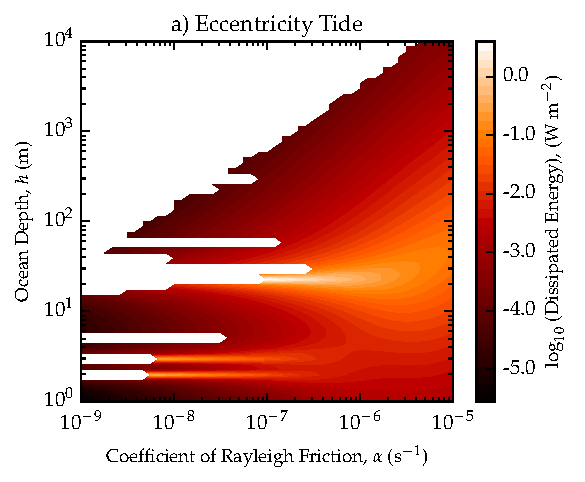
\includegraphics[width=\linewidth]{Figures/Eccentricity_RayleighFric}
%\subcaption{\label{fig:rayleighFricEcc}}
%\end{subfigure}%
%\begin{subfigure}{0.48\linewidth}
%\centering
%\includegraphics[width=\linewidth]{Figures/Obliquity_RayleighFric}
%\subcaption{\label{fig:rayleighFricObliq}}
%\end{subfigure}
%\vspace*{-0.8cm}
%\caption{Log of the average dissipated energy assuming Rayleigh (linear) friction for the eccentricity and obliquity tides. \label{fig:rayleighFric}}
%\end{figure*}

\subsection{Bottom Friction \label{subsec:result_bottom}}

\begin{figure*}[!t]
\centering
\begin{subfigure}{0.48\linewidth}
\centering
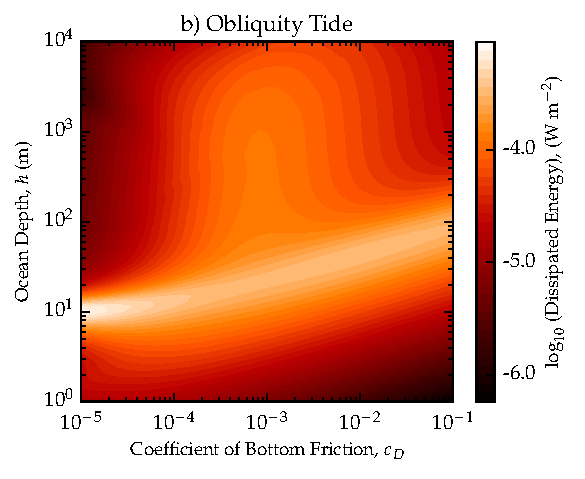
\includegraphics[width=\linewidth]{Figures/Obliquity_BottomFric}
\subcaption{\label{fig:bottomFricEcc}}
\end{subfigure}%
\begin{subfigure}{0.48\linewidth}
\centering
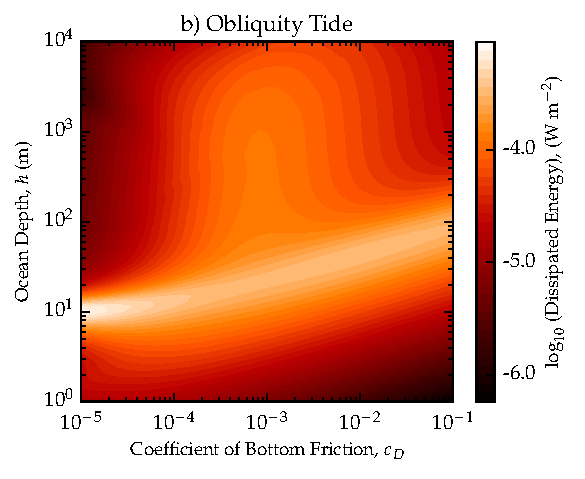
\includegraphics[width=\linewidth]{Figures/Obliquity_BottomFric}
\subcaption{\label{fig:bottomFricObliq}}
\end{subfigure}
\vspace*{-0.8cm}
\caption{Log of the average dissipated energy assuming bottom (quadratic) friction for the eccentricity and obliquity tides. \label{fig:bottomFric}}
\end{figure*}

\subsection{Scaling Laws \label{subsec:scaling}}